\chapter{Vooronderzoek en resultaten}

In dit hoofdstuk wordt er een introductie gegeven in het Blockchain domein. Deze kennis is benodigd om het onderzoek uit te voeren en om het Proof of Concept te realiseren. Daarnaast zal deze kennis helpen om de uitvoering van de opdracht te begrijpen. Het vooronderzoek dient tevens om overeenstemming te krijgen met de opdrachtgever over de richting van het onderzoek. Zoals verteld in de aanpak zijn er weinig eisen gesteld aan de uitvoering en toepassing van de afstudeeropdracht, waardoor het wenselijk is om een gezamenlijke overeenstemming te krijgen van wat mogelijk is met het onderzoek. 

Het vooronderzoek betreft kwalitatief-, exploratief onderzoek dat uitgevoerd wordt door middel van deskresearch. Om de vragen te beantwoorden is er gebruikgemaakt van zowel blogs en websites en is ervoor gekozen om de definities welke in het vooronderzoek voorkomen te beschrijven vanuit het Bitcoin protocol, zoals beschreven door \cite{nakamoto2008bitcoin}. Om de technische kennis te versterken voor de realisatie van het Proof of Concept is er een Coursera course gevolgd, Bitcoin and Cryptocurrency Technologies, waarin het Bitcoin protocol uitgelegd wordt. Dit is gevolgd omdat de beschrijving van het Bitcoin protocol niet meer toereikend is naar de huidige staat van de implementatie.

Er wordt ingegaan op de basis van Blockchain technologie waarna er gekeken wordt naar de mogelijke toepassingen. Vervolgens komt de architectuur van een Blockchain aan bod, waarbij de vraag ``Uit welke componenten bestaat een Blockchain implementatie?" wordt behandeld. Om een afbakening te maken voor het onderzoek wordt er gekeken naar wat de onderdelen Distributed Network en Identity Management bevatten. Concreet staan de vragen die behandeld worden in het vooronderzoek hieronder weergegeven.

\begin{enumerate}[noitemsep]
  \item Wat is Blockchain technologie?
  \item Waarvoor wordt Blockchain technologie gebruikt?
  \item Uit welke onderdelen bestaat een Blockchain?
  \item Waaruit bestaat het onderdeel Distributed Network binnen Blockchain technologie?
  \item Waaruit bestaat het onderdeel Identity Management binnen Blockchain technologie?
\end{enumerate}

\newpage
\section{Blockchain}
\label{chapter:blockchain}

\textit{
  In dit hoofdstuk wordt de vraag  ``Wat is Blockchain technologie?" behandeld. Het betreft het vergaren van kennis over de basis van het Blockchain begrip waarbij er ingegaan wordt op wat Blockchain is en welke eigenschappen het heeft. Door het beantwoorden van deze vraag wordt er een definitie vastgesteld van Blockchain technologie die gebruikt wordt in het gehele verslag.
}

Een blockchain is een gedistribueerde database die bestaat uit een keten van in de computer of op internet vastgelegde en samengevoegde gegevens genaamd blocks. Om deze reden wordt blockchain technologie ook wel vergeleken met een grootboek. In zekere mate is dit correct maar het omschrijft niet het meest vooraanstaande aspect van blockchain, namelijk dat het gedecentraliseerd opereert.

Om de analogie voort te zetten; een grootboek is in handen van één organisatie waarin transacties van of naar de organisatie vastgelegd worden. Dit betekent dat er een centrale autoriteit is die kan bepalen of er überhaupt wel transacties plaatsvinden, of erger, het systeem buiten gebruik kan stellen. Daarnaast is de centrale autoriteit ook in staat misbruik te maken door bijvoorbeeld transacties te registreren naar de eigenaar van het grootboek. Dit brengt een risico met zich mee die blockchain technologie oplost door het grootboek te verspreiden over een netwerk dat ervoor zorgt dat deze centrale autoriteit niet meer nodig is.

Een traditionele blockchain is weergegeven in fig. \ref{blockchain_reference}. De keten van gegevens wordt bepaald door de volgorde waarin de gegevens zijn toegevoegd. Er is daarbij een eenvoudig te controleren systeem volgens welke voorafgaande blokken aan elkaar gerelateerd behoren te zijn. Door de inhoud van het vorige block crypto grafisch te versleutelen (ook wel hashen genoemd) en deze sleutel op te nemen in een opeenvolgend blok wordt ervoor gezorgd dat gegevens van eerdere blokken niet meer gemuteerd kunnen worden. Wanneer dit wel gebeurt zou de ketting verbroken worden omdat er een nieuwe sleutel gegenereerd wordt en opeenvolgende blokken zullen refereren naar een foutieve sleutel.
  
\begin{figure}[h]
  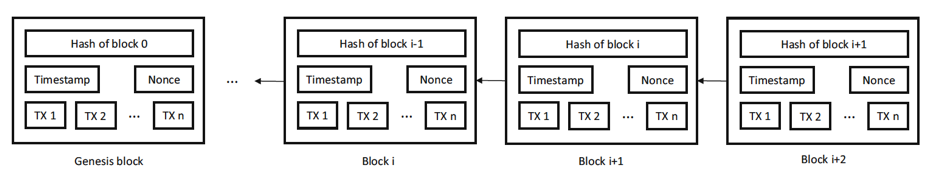
\includegraphics[width=1\textwidth]{figures/blockchain}
  \caption{Voorbeeld van een blockchain \citep{zheng2016blockchain}}
  \label{blockchain_reference}
\end{figure}

\clearpage
\subsection{Eigenschappen}

\cite{zheng2017overview}[Key Characteristics of Blockchain, p.5] stelt dat er vier eigenschappen zijn die een Blockchain definiëren:

\paragraph{Decentralisatie} In traditionele gecentraliseerde transactie systemen wordt iedere transactie gevalideerd door een centrale vertrouwde organisatie (e.g.\ banken), waardoor er een bottleneck gecreëerd wordt door de transacties te verwerken door centrale informatiesystemen. In contrast daarmee is een derde partij niet meer nodig in blockchain systemen. Consensus algoritmes zorgen ervoor dat data consistent is binnen het netwerk.

\paragraph{Persisentie} Transacties kunnen snel gevalideerd worden en invalide transacties zullen niet toegelaten worden. Het is bijna onmogelijk om te transacties verwijderen of ongedaan te maken als ze zijn opgenomen in de blockchain.

\paragraph{Anonimiteit} Elke gebruiker van het systeem kan interacteren zonder zijn ``echte" identiteit kenbaar te maken.

\paragraph{Controleerbaarheid} In bitcoin wordt de balans van een gebruiker opgeslagen door gebruik te maken van het Unspent Transaction Output (UTXO) model. Elke transactie refereert naar eerdere unspent transacties. Wanneer de huidige transactie is opgenomen in de blockchain, zal de staat van alle gerefereerde transacties verandert worden van ``unspent" naar ``spent". Hierdoor zijn transacties makkelijk te valideren en te traceren.

\newpage
\section{Toepassing}

\textit{In dit hoofdstuk wordt de vraag ``Waarvoor wordt Blockchain technologie gebruikt?'' beantwoord. Deze vraag is opgesteld omdat er geen toepassing bekend is voor de te realiseren Blockchain onderdelen, zoals aangegeven in de beschrijving van de aanpak. Het antwoord op deze vraag dient om de opdrachtgever te informeren in wat er mogelijk is met Blockchain technologie om zo een toepassing te kiezen voor het te ontwikkelen Proof of Concept. \\ \\ Er is in het bijzonder aandacht geschonken aan Blockchain als development platform aangezien de opdrachtomschrijving, bijlage \ref{appendix:opdrachtformulering}, spreekt over de realisatie van het onderdeel Smart Contract. Uitleg over het onderdeel \glspl{smart_contract} is beperkt gebleven aangezien het buiten de scope van de opdracht valt.
}

Blockchain technologie wordt steeds vaker toegepast voor het opzetten van een gedecentraliseerd systeem. Aangezien de bekendste toepassing van blockchain technologie een financieel systeem is wordt het vaak gezien als technologie die specifiek bedoeld is om financiële diensten te ondersteunen. In de literatuur wordt er echter veel geëxperimenteerd en gespeculeerd over andere mogelijke toepassingen van blockchain technologie.

\begin{wrapfigure}{r}{0.5\textwidth}
  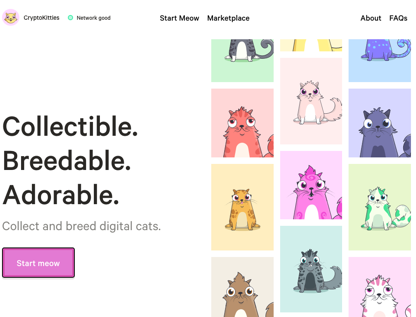
\includegraphics{figures/cryptokitties}
  \caption{CryptoKitties, een spel dat gebruik maakt van Blockchain technologie.}
  \label{cryptokitties}
\end{wrapfigure}

Zo stelt \citeauthor{atzori2015blockchain}, (\citeyear{atzori2015blockchain}) bijvoorbeeld dat blockchain technologie ingezet kan worden om de politiek en de maatschappij te veranderen. In een andere studie gedaan door \citeauthor{crosby2016blockchain}, (\citeyear{crosby2016blockchain}) wordt er onderscheid gemaakt tussen financiële en niet-financiële toepassingen die mogelijk veranderd kunnen worden door blockchain technologie. Een aantal voorbeelden die gegeven worden zijn de toepassingen bij verzekeringen, gedecentraliseerde opslag en domeinregistratie. In fig. \ref{cryptokitties} is een afbeelding te zien van de website van CryptoKitties, een van de eerste spellen die gebruik maakt van blockchain technologie, namelijk het Ethereum netwerk.

\clearpage
\subsection{Ontwikkelplatform}
Blockchains als Ethereum, EOS en HyperLedger bieden hun functionaliteit aan als development platform. Het stelt ontwikkelaars in staat om hun eigen toepassingen te realiseren, zogenaamde \gls{dapps}.

\begin{lstlisting}[
  linewidth=\textwidth, breaklines=true, 
  basicstyle=\small, label={smart_contract},
  caption={Smart contract voor ``The Greeter'' geschreven in Solidity, zoals gepresenteerd in een tutorial voor Smart Contracts op het Ethereum netwerk \citep{ethereum_smart_contract}.}]
  contract Mortal {
    /* Define variable owner of the type address */
    address owner;

    /* This function is executed at initialization and sets the owner of the contract */
    function Mortal() { owner = msg.sender; }

    /* Function to recover the funds on the contract */
    function kill() { if (msg.sender == owner) selfdestruct(owner); }
  }

  contract Greeter is Mortal {
    /* Define variable greeting of the type string */
    string greeting;

    /* This runs when the contract is executed */
    function Greeter(string _greeting) public {
        greeting = _greeting;
    }

    /* Main function */
    function greet() constant returns (string) {
        return greeting;
    }
  }
\end{lstlisting}

Door het gebruik van \glspl{smart_contract}, te zien in fig. \ref{smart_contract}, is het mogelijk om functionaliteit bij transacties te voegen om extra handelingen, die niet gerelateerd zijn tot de kern van een Blockchain implementatie, uit te voeren. Hieronder is een voorbeeld gegeven wat er mogelijk is met betrekking tot \gls{dapps}.

\paragraph{CryptoKitties} is een spel dat gebruikt maakt van het Ethereum platform, bestaand uit verzamelbare en fokbare digitale katten. De uitwisseling en het fokken van CryptoKitties wordt vastgelegd in het Ethereum netwerk door middel van \glspl{smart_contract}. Wanneer twee CryptoKitties gefokt worden, wordt het uiterlijk en de eigenschappen van hun nageslacht bepaald door het 256-bits genoom van elke ouder en een toeval element, wat leidt tot 4 miljard mogelijke genetische variaties \citep{cryptokitties}.


\newpage
\section{Architectuur}
\label{chapter:architecture}

\textit{
  In dit hoofdstuk wordt de vraag ``Uit welke componenten bestaat een Blockchain implementatie?'' behandeld. Het antwoord op deze vraag dient om een duidelijk beeld te scheppen welke componenten betrekking hebben op de onderdelen Distributed Network en Identity Management en tevens gebruikt zal worden als afstemming met zowel de opdrachtgever als de medeafstudeerder, Kevin Bos. 
}

\begin{wrapfigure}{r}{0.5\textwidth}
  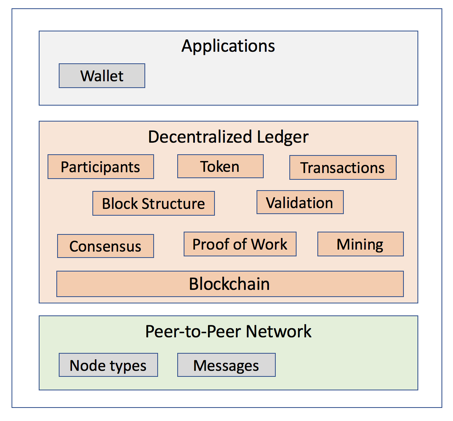
\includegraphics{figures/blockchain_architecture}
  \caption{Blockchain architectuur.}
  \label{blockchain_architecture}
\end{wrapfigure}

In fig. \ref{blockchain_architecture} is een overzicht weergegeven van de onderdelen en componenten waaruit een Blockchain bestaat. In de applicatie laag is de wallet te vinden die een gebruiker van de Blockchain doorgaans gebruikt om transacties te verrichten. De onderliggende functionaliteit van de wallet doet niets meer als het bijhouden van public- en private keys van de gebruiker waarop de nog niet uitgegeven tokens (cryptocurrency, contracten, diensten) geregistreerd staan.

De Decentralized Ledger is de kern van de technologie en zorgt ervoor dat de globale blockchain consistent en fraudebestending blijft. De fundamentele structuur achter de gehele technologie is de blockchain, waar transacties gegroepeerd worden in blokken en elk blok crypto grafisch verbonden wordt met het vorige blok. Een transactie is een vorm van uitwisseling van tokens tussen deelnemers, ook wel nodes genoemd, van het systeem. Voordat transacties als valide worden beschouwd, ondergaan ze een validatie proces die uitgevoerd wordt door alle nodes in het systeem. Het proces van het groeperen van transacties in een blok dat toegevoegd wordt aan het einde van de blockchain wordt ook wel minen genoemd. Om er zeker van te zijn dat er overeenstemming is onder alle deelnemers over welke blockchain legitiem is, wordt er gebruik gemaakt van een Proof-of-Work algoritme tijdens het mining proces om te bepalen welke ketting de meeste inspanning vereist.

Het laatste component is het peer-to-peer netwerk, waarin verschillende node types gedefinieerd zijn. Zo heb je bijvoorbeeld de validatie node die transacties valideert en een mining node die het mining process uitvoert. Om de Decentralized Ledger bij te werken en te onderhouden communiceren de nodes met elkaar door middel van het versturen van berichten.

\newpage
\section{Gedistribueerd netwerk}

\textit{
  In dit hoofdstuk wordt de vraag ``Waaruit bestaat het onderdeel gedistribueerd netwerk binnen Blockchain technologie?'' behandeld. Bij deze vraag wordt er gekeken naar de geïdentificeerde onderdelen uit hoofdstuk \ref{chapter:architecture}. Er wordt een korte introductie gegeven in peer-to-peer netwerken en waarom het een belangrijk onderdeel is bij het realiseren van de eigenschappen, behandeld in hoofdstuk \ref{chapter:blockchain}, van een Blockchain implementatie. Het antwoord op deze vraag zal helpen bij het selecteren van zoektermen die gebruikt worden om inventarisatie te doen op de onderdelen die het Distributed Network omvat.
}

Het onderdeel Distributed Network bestaat uit het verspreiden, uitbreiden en het behalen van consensus over de staat van de Blockchain tussen de deelnemers aan het netwerk. Om dit te doen wordt er gebruik gemaakt van een \acrfull{P2P} implementatie waarbij het mogelijk is om een lokale versie van de ketting aan te bieden aan andere nodes binnen het \acrshort{P2P} netwerk, om zo de huidige chain up-to-date te houden met wijzigingen die gedaan zijn door de verschillende verbonden nodes. Dit leidt tot een complex probleem dat beschreven wordt als het Byzantine Generals Problem \citep{lamport1982byzantine}, wat beschrijft aan de hand van een abstract voorbeeld dat het essentieel is voor een betrouwbaar computersysteem om te kunnen gaan met fouten die optreden in een of meer van de componenten, waardoor het kan voorkomen dat er conflicterende informatie verstuurd wordt naar de andere componenten van het systeem.

\textbf{Peer-to-Peer}

De term \acrshort{P2P} betekend dat alle computers die deel uit maken van het netwerk, peers van elkaar zijn, gelijk aan elkaar zijn, er geen speciale "nodes" zijn en dat alle deelnemers in het netwerk de last delen van het leveren van netwerkdiensten \citep[~p.171]{Antonopoulos:2014:MBU:2695500}. Het is een techniek die cruciaal is voor Blockchain en de doelen die het probeert te behalen. \acrshort{P2P} systemen verdelen namelijk de kosten om data te delen – opslag voor bestanden en bandbreedte voor het versturen van de bestanden – over de deelnemers van het netwerk, waardoor applicaties kunnen schalen zonder krachtige, dure servers \citep{bawa2003peer}.

Een van de bekendste toepassingen van een peer-to-peer netwerk is het creëren van een gedecentralizeerd file-sharing protocol. Implementaties hiervan zijn BitTorrent, LimeWire en Gnutella. Om een bestand te distribueren wordt het opgesplitst in delen, waarbij er een hash gecreëerd wordt voor elk deel. Wanneer een andere deelnemer van het netwerk een deel ontvangt wordt er gekeken aan de hand van de hash of het onderdeel geen fouten bevat. Bestanden worden geregistreerd in het netwerk door het opnemen van de hashes in een zogenaamde \textit{tracker} die gebruik maakt van een \acrfull{DHT}. Een voorbeeld van een DHT is te zien in fig. \ref{DHT}.

\newpage
\begin{wrapfigure}{l}{0.6\textwidth}
  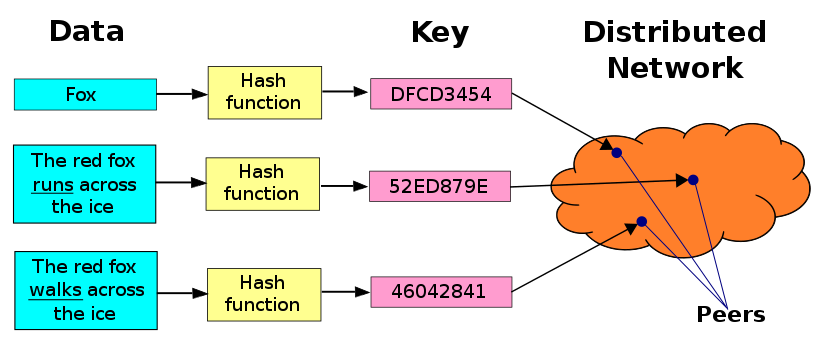
\includegraphics[width=0.6\textwidth]{figures/DHT}
  \caption[Distributed Hash Table] {
    Door het vertalen van data naar een cryptografische sleutel is het mogelijk om aan de hand van de sleutel de data op te vragen aan peers die de data bezitten.
  }
  \label{DHT}
\end{wrapfigure}

\textbf{Consensus}

Consensus is een dynamische manier van het behalen van overeenstemming in een groep. In blockchain implementaties wordt het gebruikt om overeenstemming te behalen over de staat van het netwerk en de volgorde waarin transacties gedaan zijn. Met het consensus algoritme wordt er een zekere mate van veiligheid gewaarborgd, waardoor het voor een kwaadwillende deelnemer (bijna) onmogelijk dient te zijn om het netwerk te beïnvloeden. Het kan voorkomen dat een kwaadwillende deelnemer probeert het netwerk te beïnvloeden waardoor er tegenstrijdige consensus kan optreden en een \gls{fork} ontstaat in het netwerk.

\textbf{Fork}

Een \gls{fork} is een splitsing in het netwerk die veroorzaakt is door een verandering in het protocol of door het toedoen van kwaadwillende deelnemer(s). Er zijn hiervoor twee categorieën \glspl{fork}, een \gls{hard_fork} en een \gls{soft_fork}.

\paragraph{Soft fork}

is een verandering in het netwerk die terugwaartse compatibiliteit heeft met eerdere versies van het protocol. Als voorbeeld kan er voor gekozen worden dat in plaats van blocks een limiet hebben van 1MB, de regel aangepast wordt zodat blocks een grootte van 500K moeten hebben. Als een \gls{soft_fork} verkeerd gaat is het nog steeds mogelijk dat er een \gls{hard_fork} optreed \citep[Soft Fork]{coindesk:forks}.

\paragraph{Hard fork}

is een protocol update waarbij een nieuwe regel geïntroduceerd wordt, waardoor het netwerk geen compatibiliteit heeft met oudere versies. Dit zorgt ervoor dat deelnemers in het netwerk die een oudere versie hebben, de nieuwe transacties als invalide beschouwen. Een voorbeeld van een regel waarbij een \gls{hard_fork} ontstaat is bijvoorbeeld het ophogen van de block grootte naar 2MB in plaats van 1MB \citep[Hard Fork]{coindesk:forks}. 

\newpage
\textbf{\Glspl{node}}

Alhoewel de structuur van een Blockchain dezelfde structuur afdwingt voor de \glspl{node} in het netwerk, kunnen zij een verschillende rol spelen. Alle \glspl{node} binnen het netwerk valideren, verspreiden en ontdekken en onderhouden connecties met andere \glspl{node} binnen het netwerk. In fig. \ref{blockchain_node_types} is te zien welke services een  \gls{full_node} in het Bitcoin netwerk aanbiedt. 

\begin{wrapfigure}{r}{0.4\textwidth}
  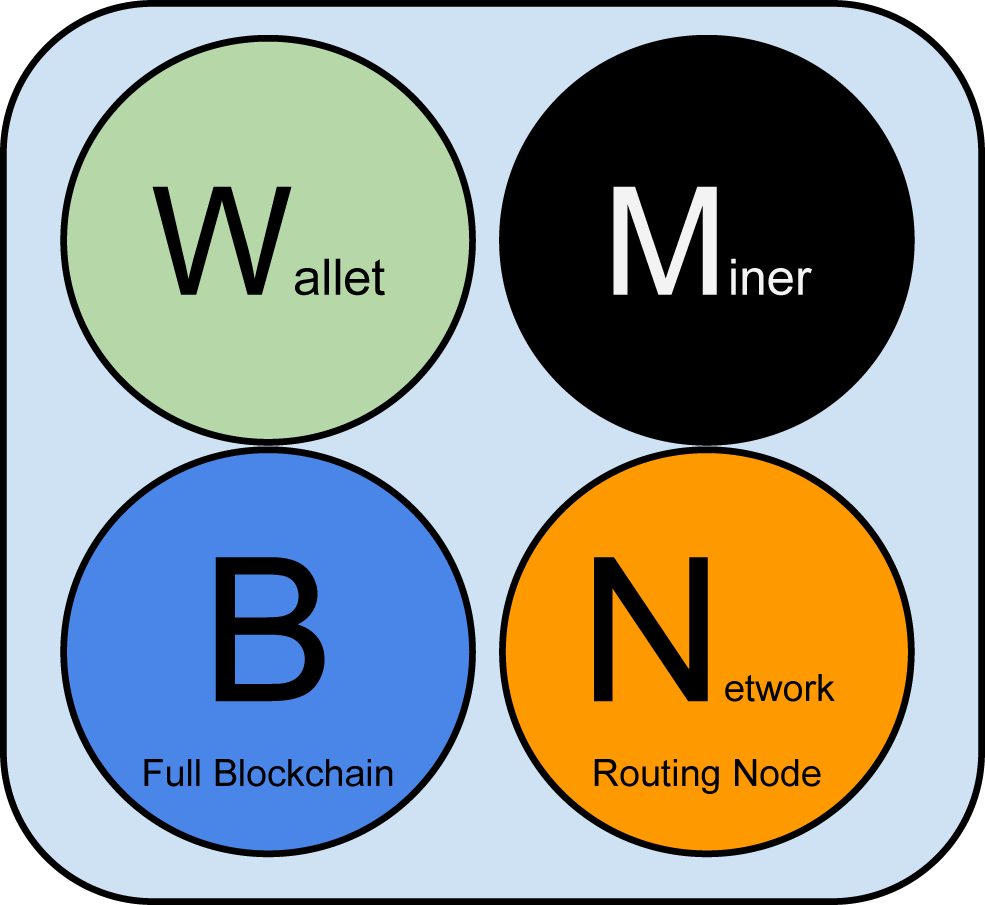
\includegraphics[width=0.4\textwidth]{figures/bitcoin_node_types}
  \caption[Bitcoin Node functionaliteiten] {
    Een bitcoin netwerk node die alle functies bevat: wallet, mining, blockchain database en netwerk routing, \citep[p.~172]{Antonopoulos:2014:MBU:2695500}.
  }
  \label{blockchain_node_types}
\end{wrapfigure}

Een \textbf{\gls{full_node}} is een collectie van functies, namelijk routing, de blockchain database, het mining proces en wallet services en bevat een gehele kopie van de actuele blockchain. Een \textbf{\gls{wallet_node}} is een deelnemer in het netwerk die een subset van de gehele blockchain bevat om transacties te versturen, verifiëren en ontvangen. De \textbf{\glspl{mining_node}} concurreren voor het creëren van een nieuw block door het uitvoeren van het Proof-of-Work algoritme. 

Alle \glspl{node} binnen het netwerk bieden gelijke diensten aan en kunnen gebruik maken van dezelfde diensten terwijl ze samenwerken door middel van een consensus protocol.

De verschillende services binnen het netwerk en de \gls{node} types die hieraan meewerken is dan ook een architecturale keuze over de indeling van het \acrshort{P2P} netwerk.


\newpage
\section{Identiteit}

\textit{
  In dit hoofdstuk wordt de vraag ``Waaruit bestaat het onderdeel Identity Management binnen Blockchain technologie?'' behandeld. Zoals beschreven in hoofdstuk \ref{chapter:blockchain} zijn anonimiteit en controleerbaarheid belangrijke eigenschappen van een Blockchain implementatie. Allereerst zal er beschreven worden wat identiteit inhoud binnen een Blockchain en welke mogelijke vormen van management er zijn. Het antwoord op deze vraag wordt gebruikt om zoektermen op te stellen en een afbakening te creëren voor de te onderzoeken protocollen.
}

In het vooronderzoek is er weinig gevonden over Identity Management en zelf wist ik dan ook niet goed wat dit onderdeel voor functionaliteiten bevat. In eerste instantie is er gekeken naar de verschillende types van Blockchain, waarbij gebruikers van het systeem autorisatie hebben tot bepaalde acties. Om een beter beeld te schetsen en de afbakening van het onderdeel compleet te maken voor het onderzoek is er besloten om een gesprek te houden met Pim Otte.

Uit dit gesprek is naar voren gekomen dat het Identity Management gedeelte gaat over hoe de Blockchain implementatie met public keys (de identiteit van een gebruiker) omgaat. Als tip werd er gegeven om te kijken naar de wallet software indien beschikbaar. Dit is software die de public- en private key beheert voor een gebruiker. Daarnaast is er ook een tip gegeven over het onderdeel Distributed Network. Om een goed beeld te krijgen van de aanvallen waar het netwerk tegen bestand is, is het handig om een threat model op te stellen.

Het onderdeel Identity Management beschrijft hoe de Blockchain omgaat met de identiteit van gebruiker die deel uitmaakt van het netwerk. Daarnaast is het mogelijk dat een bepaald type Blockchain meer doet dan alleen de identiteit van de gebruiker beheerd of maskeert. 

\subsection{Categorieën}

\cite{zheng2017overview} deelt Blockchain implementaties op in drie categorieën, waarin de zichtbaarheid en participatie in het consensus proces gelimiteerd.

\paragraph{Public} In een public Blockchain zijn alle transacties publiekelijk inzichtbaar en iedereen in het netwerk maakt onderdeel uit van het consensus proces. Dit wordt ook wel gezien als een permissionless Blockchain.

\paragraph{Consortium} In een consortium Blockchain is er een groep van vooraf geselecteerde nodes die deel uitmaken van het consensus proces. De consortium Blockchain wordt meestal gebruikt door meerdere organisaties en is gedeeltelijk gedecentraliseerd. Omdat bepaalde nodes geïdentificeerd dienen te worden wordt dit type Blockchain gezien als een permissioned Blockchain.

\clearpage
\paragraph{Private} In een private Blockchain worden alleen nodes van een specifieke organisatie toegelaten tot het consensus proces. Het wordt ook wel als een centraal netwerk gezien omdat het in volledige controle is van één organisatie. Omdat het hier gaat om volledige restrictie tot het Blockchain netwerk wordt dit type Blockchain gezien als een permissioned Blockchain.

In een consortium en een private Blockchain dient de gebruiker zich te identificeren aan de hand van een identiteit. Zoals eerder vermeld maakt Blockchain gebruik van een public- en private keys om de gebruiker te identificeren. Dit hanteert in zekere mate een permissie model waarbij de autorisatie van een gebruiker vastgelegd word aan de hand van de identificatie (i.e.\ de public key) die het netwerk gebruikt.

\subsection{Identificatie}

Identificatie wordt doorgaans gedaan aan de hand van een public key van een gebruiker. Een van de missies van Blockchain is totale anonimiteit, alleen zijn er een aantal problemen die volledige anonimiteit tegengaan. Om de terminologie duidelijk te maken wordt hieronder het verschil tussen pseudoniem en anoniem uitgelegd aan de hand van voorbeelden vanuit het Bitcoin protocol.

\begin{formal}
  ``Anonymity is the state of being not identifiable within a set of subjects, the anonymity set."
  \\ \cite{pfitzmann2001anonymity}.
\end{formal}

\paragraph{Pseudoniem} 

Bij een pseudoniem gaat er om een referentie naar de identiteit. 

\paragraph{Anoniem}







\newpage
\section{Obstakels}

In het vooronderzoek is er weinig gevonden over Identity Management en zelf wist ik dan ook niet goed wat dit onderdeel voor functionaliteiten bevat. In eerste instantie is er gekeken naar de verschillende types van Blockchain, waarbij gebruikers van het systeem autorisatie hebben tot bepaalde acties. Om een beter beeld te schetsen en de afbakening van het onderdeel compleet te maken voor het onderzoek is er besloten om een gesprek te houden met de Blockchain Expert.

Uit dit gesprek is naar voren gekomen dat het Identity Management gedeelte gaat over hoe de Blockchain implementatie met public keys (de identiteit van een gebruiker) omgaat. Als tip werd er gegeven om te kijken naar de wallet software indien beschikbaar. Dit is software die de public- en private key beheert voor een gebruiker. Daarnaast is er ook een tip gegeven over het onderdeel Distributed Network. Om een goed beeld te krijgen van de aanvallen waar het netwerk tegen bestand is, is het handig om een threat model op te stellen.

\newpage
\section{Conclusie}

Naar aanleiding van de resultaten uit het vooronderzoek zijn er keuzes gemaakt die zich reflecteren in het onderzoek. Hieronder is per vraag beschreven over de implicaties die de resultaten gaven tegenover het onderzoek. 

Uit de vraag ``Waaruit bestaat het onderdeel Distributed Network binnen Blockchain technologie?'' is gebleken dat het consensus proces invloed heeft op de structuur van het netwerk. Het soort consensus zal dan ook gebruikt worden om de verschillende type Distributed Networks te onderscheiden. Ook zullen de verschillende type van nodes onderzocht worden om te identificeren welke bijdrage een bepaald type node levert om het netwerk in stand te houden. 

In de resultaten van de vraag ``Waaruit bestaat het onderdeel Identity Management binnen Blockchain technologie?'' is er geïdentificeerd dat er twee manieren zijn waarop de privacy van de gebruiker gewaarborgd wordt, namelijk of het een permissionless of permissioned Blockchain is en de identificatie van de gebruiker binnen het netwerk. Er wordt aangegeven dat het niveau van privacy en autorisatie ligt aan de categorie van waar de Blockchain deel van uitmaakt.

\begin{enumerate}[noitemsep]
  \item Zichtbaarheid van acties die de gebruiker onderneemt op de Blockchain.
  \item Autorisaties voor acties die de gebruiker wilt ondernemen op de Blockchain.
\end{enumerate}
